\documentclass[10pt,twocolumn,letterpaper]{article}
\usepackage[review]{cvpr}

\usepackage{amsmath,amssymb,mathtools}
\usepackage{booktabs}
\usepackage{multirow}
\usepackage{tabularx}
\usepackage{graphicx}
\usepackage[dvipsnames]{xcolor}
\usepackage{tikz}
\usetikzlibrary{arrows.meta,positioning,fit,calc,shapes.geometric,decorations.pathreplacing}
\usepackage{algorithm}
\usepackage{algpseudocode}
\usepackage[numbers,sort&compress]{natbib}
\usepackage[colorlinks=true,linkcolor=MidnightBlue,citecolor=MidnightBlue,urlcolor=MidnightBlue]{hyperref}
\usepackage[capitalize,nameinlink]{cleveref}

% Shared notation for DUCA-TAD.
\newcommand{\R}{\mathbb{R}}
\newcommand{\E}{\mathbb{E}}
\newcommand{\VideoWin}{\mathcal{V}}
\newcommand{\Detector}{\mathcal{D}}
\newcommand{\Acquirer}{\mathcal{A}}
\newcommand{\Ssel}{\mathcal{S}}
\newcommand{\Grid}{\mathcal{G}}
\newcommand{\Lledger}{\mathcal{L}}
\newcommand{\Bbudget}{\mathcal{B}}
\newcommand{\Tdense}{T}
\newcommand{\Ksel}{K}
\newcommand{\Kmain}{K_{\mathrm{main}}}
\newcommand{\pact}{p_{\mathrm{act}}}
\newcommand{\pzs}{p_{\mathrm{zs}}}
\newcommand{\putil}{u}
\newcommand{\prisk}{r}
\newcommand{\pred}{\rho}
\newcommand{\taucoord}{\tau}
\newcommand{\Mmask}{m}
\newcommand{\thet}{\theta}
\newcommand{\etaopt}{\eta}
\newcommand{\philo}{\phi_{\mathrm{low}}}
\DeclareMathOperator*{\argmax}{arg\,max}
\DeclareMathOperator*{\argmin}{arg\,min}


\title{DUCA-TAD: Detector-Utility-Calibrated In-Forward Temporal Acquisition for Efficient Temporal Action Detection}

\author{Anonymous CVPR Submission\\
Paper ID: ****}

\begin{document}

\maketitle

\begin{abstract}
Temporal action detection (TAD) is expensive because high-quality detectors consume long temporal windows while remaining sensitive to start and end boundaries. We study a stricter problem than offline frame subsampling: an acquisition plugin must run in the detector forward path, hard-select at most 384 observations from a dense candidate window, and preserve the original temporal coordinate system used for localization. We call this setting \emph{in-forward} or \emph{window-online} acquisition: the decision is computed on the current detector window rather than loaded from a precomputed ledger, but it is not a causal streaming claim. We propose DUCA-TAD, a detector-utility-calibrated acquisition plugin for AdaTAD/ActionFormer-style detectors. DUCA-TAD uses deploy-visible signals, including zero-shot actionness, motion or feature energy, and optional learned probes, to score candidate observations. Training uses dense detector utility only as supervision: a warm-up stage calibrates the selector with train-only detector responsibility, boundary support, and hard-negative risk, and a hard-forward surrogate fine-tuning stage keeps the detector input sparse while updating the selector through explicit utility and coverage losses. At inference time, the graph contains no teacher, ground truth, raw prediction cache, or offline decision ledger. The selector emits original-time selected positions and a sparse temporal grid; an audit ledger is written only for reproducibility and leakage checks. We define the method contract and an evaluation protocol covering zero-shot actionness diagnostics, selection geometry, sparse detector mAP, high-tIoU boundary diagnostics, and no-leak compute accounting.
\end{abstract}

\section{Introduction}

Temporal action detection (TAD) asks a model to classify action instances and localize their temporal boundaries in long, untrimmed videos. Recent detectors improve this task with stronger temporal heads, boundary modeling, and large video backbones \citep{zhang2022actionformer,shi2023tridet,liu2024adatad}. The cost of this progress is direct: the detector must process dense temporal evidence even though many observations are background, repeated action interiors, or low-value context.

Efficient TAD cannot be reduced to generic frame sampling. Uniform sampling is simple, but it allocates the same budget to empty windows and boundary-dense windows. Actionness top-$K$ is more task-aware, but it tends to keep confident action interiors and can discard the low-confidence transitions that determine high-tIoU localization. The target problem is therefore \emph{in-forward detector acquisition}: for each detector window, choose which original-time observations the detector should actually consume under a hard budget.

We propose \textbf{DUCA-TAD}, a detector-utility-calibrated in-forward temporal acquisition plugin. DUCA-TAD is not a new TAD detector and not an offline ledger pipeline. It is a selector/adapter inserted before AdaTAD-, ActionFormer-, or similar TAD detectors. Given a dense candidate window, typically $T=768$, DUCA hard-selects at most $\Kmain=384$ original-time positions. The detector consumes only those selected observations, while sparse coordinate metadata maps selected-axis predictions back to original video time. We use \emph{in-forward} and \emph{window-online} to mean that the selector runs on the current detector window during the forward path; the paper does not claim prefix-causal streaming or delayed online emission.

The plugin separates three information regimes. During training, dense detector responsibility, boundary support, localization loss, and hard-negative risk may supervise the acquisition module. During hard-forward fine-tuning, the detector still receives a packed sparse subset, while the selector is updated by explicit utility, boundary, hole, and coverage losses computed on the same training windows. During validation and deployment, selection uses only deploy-visible inputs such as zero-shot actionness, motion or feature energy, and optional learned probes. No teacher utility, ground truth, detector raw prediction, prediction cache, or offline decision ledger is read at inference.

\begin{figure*}[t]
\centering
\resizebox{0.98\textwidth}{!}{%
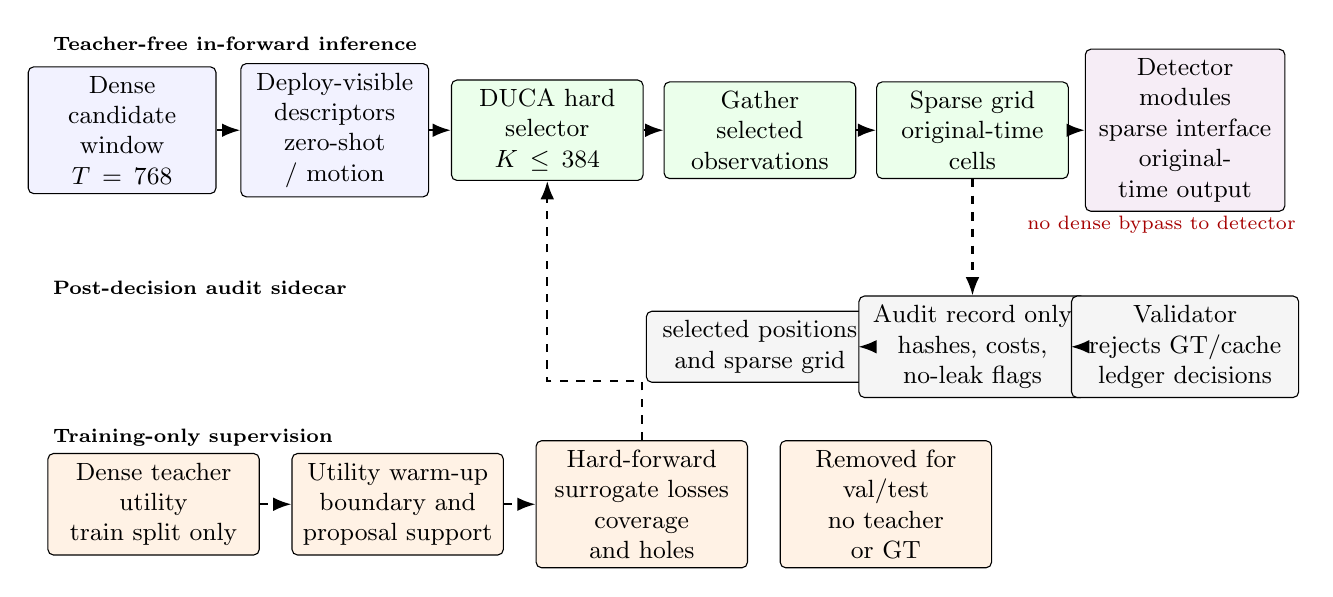
\begin{tikzpicture}[
    font=\small,
    node distance=0.55cm and 0.70cm,
    source/.style={draw, rounded corners=2pt, align=center, minimum height=0.82cm, text width=2.15cm, fill=blue!5},
    plugin/.style={draw, rounded corners=2pt, align=center, minimum height=0.82cm, text width=2.20cm, fill=green!8},
    det/.style={draw, rounded corners=2pt, align=center, minimum height=0.82cm, text width=2.30cm, fill=violet!7},
    train/.style={draw, rounded corners=2pt, align=center, minimum height=0.74cm, text width=2.45cm, fill=orange!10},
    audit/.style={draw, rounded corners=2pt, align=center, minimum height=0.74cm, text width=2.65cm, fill=gray!8},
    arrow/.style={-Latex, thick},
    dashedarrow/.style={-Latex, thick, dashed},
    stoparrow/.style={-Latex, thick, dashed, red!65!black},
    note/.style={align=center, font=\scriptsize}
]

\node[note, anchor=west] at (-6.95,2.65) {\textbf{Teacher-free in-forward inference}};
\node[source] (dense) at (-5.95,1.55) {Dense candidate\\window\\$T=768$};
\node[source] (src) at (-3.25,1.55) {Deploy-visible\\descriptors\\zero-shot / motion};
\node[plugin] (selector) at (-0.55,1.55) {DUCA hard\\selector\\$\Ksel\le384$};
\node[plugin] (gather) at (2.15,1.55) {Gather\\selected\\observations};
\node[plugin] (grid) at (4.85,1.55) {Sparse grid\\original-time\\cells};
\node[det] (detector) at (7.55,1.55) {Detector modules\\sparse interface\\original-time output};

\draw[arrow] (dense) -- (src);
\draw[arrow] (src) -- (selector);
\draw[arrow] (selector) -- (gather);
\draw[arrow] (gather) -- (grid);
\draw[arrow] (grid) -- (detector);
\node[note, text=red!65!black] at (7.25,0.35) {no dense bypass to detector};

\node[note, anchor=west] at (-6.95,-0.45) {\textbf{Post-decision audit sidecar}};
\node[audit] (auditin) at (2.15,-1.20) {selected positions\\and sparse grid};
\node[audit] (audit) at (4.85,-1.20) {Audit record only\\hashes, costs,\\no-leak flags};
\node[audit] (validator) at (7.55,-1.20) {Validator\\rejects GT/cache\\ledger decisions};
\draw[dashedarrow] (grid.south) -- (audit.north);
\draw[dashedarrow] (auditin) -- (audit);
\draw[dashedarrow] (audit) -- (validator);

\node[note, anchor=west] at (-6.95,-2.35) {\textbf{Training-only supervision}};
\node[train] (teacher) at (-5.55,-3.20) {Dense teacher\\utility\\train split only};
\node[train] (warm) at (-2.45,-3.20) {Utility warm-up\\boundary and\\proposal support};
\node[train] (surrogate) at (0.65,-3.20) {Hard-forward\\surrogate losses\\coverage and holes};
\node[train] (forbid) at (3.75,-3.20) {Removed for\\val/test\\no teacher or GT};

\draw[dashedarrow] (teacher) -- (warm);
\draw[dashedarrow] (warm) -- (surrogate);
\draw[dashedarrow] (surrogate.north) -- ++(0,0.75) -| (selector.south);

\end{tikzpicture}}
\caption{\textbf{DUCA-TAD in-forward acquisition plugin.} During inference, deploy-visible descriptors feed a hard selector that chooses at most 384 original-time observations for the detector forward path. The detector consumes the gathered sparse observations, while a sparse grid carries original-time cells for assignment, decoding, NMS, and evaluation. Training-only teacher utility supervises warm-up and surrogate coverage losses, but teacher payloads, ground truth, caches, and offline ledger decisions are absent from validation and deployment. The audit sidecar is written after selection and has no arrow back into the decision graph.}
\label{fig:architecture}
\end{figure*}


\cref{fig:architecture} shows the resulting contract. The selector emits hard \texttt{selected\_positions}; the sparse temporal grid carries their original dense indices and support cells; the audit ledger is written after the in-forward decision for reproducibility and leakage checks. This distinction matters because a precomputed ledger can hide oracle information, and selected-rank time can distort boundaries even when recognition remains strong.

This paper makes four contributions.

\begin{itemize}
    \item We formulate in-forward sparse acquisition for TAD as a hard-budget plugin contract: the detector consumes $\Ksel\le384$ selected observations, and all proposals are decoded in original time.
    \item We introduce DUCA-TAD, an acquisition module trained by detector-utility warm-up and hard-forward surrogate fine-tuning, while remaining teacher-free at inference.
    \item We incorporate zero-shot actionness as a deploy-visible branch and evaluation target, separating coarse action/background quality from selection geometry and final detector mAP.
    \item We define an audit and evaluation protocol covering no-leak provenance, compute accounting, boundary diagnostics, matched-budget baselines, and high-tIoU sparse detector performance.
\end{itemize}

\section{Related Work}

\paragraph{Temporal action detection.}
TAD methods have progressed from proposal generation to dense one-stage localization. BMN models boundary matching for proposals \citep{lin2019bmn}, G-TAD propagates context over temporal graphs \citep{xu2020gtad}, ActionFormer uses anchor-free transformer heads over temporal feature pyramids \citep{zhang2022actionformer}, and TriDet emphasizes relative boundary modeling \citep{shi2023tridet}. OpenTAD highlights how much standardized implementation details affect fair TAD comparisons \citep{liu2025opentad}. DUCA-TAD does not replace these detectors. It addresses the preceding acquisition question: which observations should a detector receive under a strict budget?

\paragraph{End-to-end and efficient TAD.}
Frozen-feature pipelines hide video-backbone cost in preprocessing, while end-to-end detectors expose that cost during training and inference. VideoMAE-style representations strengthen video backbones \citep{tong2022videomae}, and AdaTAD adapts large backbones for long-window TAD \citep{liu2024adatad}. Efficiency-oriented TAD has studied sampling-aware end-to-end training \citep{liu2023etad} and detector compression by progressive block dropping \citep{chen2025progressiveblockdrop}. DUCA-TAD is complementary: it keeps the detector architecture reusable but makes sparse input coordinates and metadata explicit.

\paragraph{Frame selection and online video reasoning.}
Video reasoning systems often select frames to fit long videos into a bounded context. Flexible Frame Selection learns frame policies for video-language reasoning \citep{buch2025flexible}, and reinforcement-learning selectors optimize long-video frame choices \citep{qin2026efficientframe}. These tasks usually ask for answers over a visual context, not boundary-accurate temporal segments. TAD acquisition must preserve original-time geometry because selected-rank time can corrupt assignment, regression, and NMS.

\paragraph{Hard subset selection.}
Top-$K$ frame selection creates a discrete interface between the acquisition policy and the downstream model. For TAD, this interface is stricter than attention or soft token weighting because the detector must actually run on the selected observations. DUCA-TAD therefore treats straight-through estimators as an implementation option that must be verified, and its main method uses hard sparse forwards with explicit surrogate utility, boundary, and coverage losses for selector training.

\paragraph{Zero-shot actionness.}
Vision-language models such as CLIP support zero-shot recognition through natural-language prompts \citep{radford2021learning}. DUCA-TAD uses this capability only as a deploy-visible actionness prior or baseline. Zero-shot action/background separation is not a TAD result: it must be evaluated first as coarse actionness, then as selection geometry, and only finally by sparse detector mAP.

\paragraph{Detector utility and provenance.}
Actionness is a useful cue, but detector utility also depends on boundary support, proposal ranking, localization loss, and hard-negative suppression. A deployable selector must not read validation labels, teacher utilities, raw detector predictions, cached proposals, or an offline oracle ledger. DUCA-TAD therefore treats the ledger as a post-decision audit record and makes the inference graph teacher-free.

\section{Problem Formulation}

\subsection{In-Forward Window Acquisition Contract}

Let a dense candidate window be
$\VideoWin=\{v_t\}_{t=1}^{\Tdense}$ with original dense-time coordinate
$\taucoord_t=t$. The main budget setting uses $\Tdense=768$ and
$\Kmain=384$. DUCA inserts an acquisition plugin in the detector forward path:
\begin{align}
    x_t &= \philo(v_t), \\
    \Ssel &= \Acquirer_{\thet}(x_{1:\Tdense})
          = \{s_1 < \cdots < s_{\Ksel}\}, \qquad
          \Ksel \le \Kmain .
    \label{eq:online_policy}
\end{align}
The detector receives only $\VideoWin_{\Ssel}$, not the full sequence. The
selected set stores original dense indices, so $\taucoord_{s_i}$ remains the
coordinate used for assignment, decoding, and evaluation. We call this setting
\emph{in-forward} or \emph{window-online}: the selection is computed from the
current detector window during the forward path and is not loaded from an
offline decision record. The setting does not require causal streaming or
prefix-only outputs.

\subsection{Observation and Compute Boundary}

The object selected by DUCA depends on where the plugin is inserted. In a
pre-backbone setting, $v_t$ is a raw clip or frame group and acquisition reduces
the cost of both the backbone and detector head. In a feature-stream setting,
$v_t$ is a precomputed temporal descriptor and acquisition reduces the cost of
the detector head and subsequent temporal processing. We therefore report
compute with separate terms for descriptor extraction, zero-shot scoring,
selector inference, backbone processing, detector head, and post-processing:
\begin{align}
    C_{\mathrm{total}}
    &=
    C_{\mathrm{desc}} + C_{\mathrm{score}} + C_{\mathrm{sel}}
    \notag\\
    &\quad
    + C_{\mathrm{backbone}}(\Ksel)
    + C_{\mathrm{head}}(\Ksel)
    + C_{\mathrm{post}} .
    \label{eq:compute_boundary}
\end{align}
This boundary prevents a frozen-feature experiment from being presented as a
full video-backbone saving.

\subsection{Teacher-Free Inference Boundary}

At validation and deployment, $x_t$ may contain only deploy-visible information:
zero-shot actionness, motion or feature energy, low-resolution descriptors, and
optional learned probes. The online decision cannot use ground truth, oracle
boundaries, teacher utility, detector raw predictions, prediction caches, or a
precomputed decision ledger. We write this as
\begin{align}
    z^{\mathrm{deploy}}_t
    &=
    (\pzs(t), e^{\mathrm{mot}}_t, e^{\mathrm{feat}}_t, p^{\mathrm{probe}}_t),
    \notag\\
    \Ssel
    &=
    \Acquirer_{\thet}(z^{\mathrm{deploy}}_{1:\Tdense}).
    \label{eq:deploy_boundary}
\end{align}
An audit ledger may record the decision after it is made, but it is not an
input to \cref{eq:online_policy}.

\subsection{Detector-Utility Target}

The selector should predict detector utility rather than actionness alone. For
training windows, a dense detector or frozen teacher defines positive detector
points $\mathcal{P}^{+}$. Each point $p$ has classification loss
$\ell^{\mathrm{cls}}_p$, localization loss $\ell^{\mathrm{loc}}_p$, ranking or
hard-negative weight $r_p$, and temporal responsibility kernel $a_{p,t}$. A
train-only utility target is
\begin{align}
    d_t &=
      \sum_{p\in\mathcal{P}^{+}}
      a_{p,t}
      (\ell^{\mathrm{cls}}_p+\ell^{\mathrm{loc}}_p+r_p),
      \notag\\
    u^{\star}_t &=
    \mathrm{norm}\!\left(
      \alpha y^{\mathrm{bnd}}_t
      + \beta y^{\mathrm{act}}_t
      + \gamma d_t
    \right).
    \label{eq:utility_target}
\end{align}
The target supervises acquisition on the training split only. It is discarded
before validation and deployment.

\subsection{Sparse Temporal Grid}

Hard selection creates a selected axis $i=1,\ldots,\Ksel$, but selected rank is
not physical time. DUCA therefore passes the detector a sparse temporal grid
\begin{equation}
    \Grid_{\Ssel}
    =
    \{(i, s_i, \taucoord_{s_i}, \ell_i, r_i)\}_{i=1}^{\Ksel},
    \label{eq:sparse_grid}
\end{equation}
where $\ell_i$ and $r_i$ are the left and right original-time support bounds of
the selected cell. With $T_{\mathrm{valid}}$ denoting the valid prefix length,
we use midpoint cells
\begin{align}
    \ell_i &=
    \begin{cases}
    1, & i=1,\\
    \frac{1}{2}(\taucoord_{s_{i-1}}+\taucoord_{s_i}), & i>1,
    \end{cases}
    \notag\\
    r_i &=
    \begin{cases}
    T_{\mathrm{valid}}, & i=\Ksel,\\
    \frac{1}{2}(\taucoord_{s_i}+\taucoord_{s_{i+1}}), & i<\Ksel.
    \end{cases}
    \label{eq:grid_cells}
\end{align}
Detector point assignment, regression range checks, offset targets, decoded
segments, and NMS are all expressed in original-time units. For a ground-truth
segment $(b^s,b^e)$ assigned to selected point $i$ with center
$c_i=\taucoord_{s_i}$, the offset target is
\begin{equation}
    \delta_i^\star=(c_i-b^s,\ b^e-c_i),
    \qquad
    \hat b^s=c_i-\hat\delta_i^L,\quad
    \hat b^e=c_i+\hat\delta_i^R .
    \label{eq:original_time_decode}
\end{equation}
If the detector predicts on the selected axis, the proposal must be remapped
through $\Grid_{\Ssel}$ before mAP is computed. This grid is the key object for
high-IoU credibility.

\section{Method}

\subsection{Overview}

DUCA-TAD is an in-forward acquisition plugin placed before a reusable TAD detector.
It has five parts: deploy-visible actionness sources, a temporal utility
selector, hard top-$K$ acquisition, an original-time sparse grid, and an audit
record. The detector architecture is reused, while sparse input coordinates and
metadata are made explicit.

\subsection{Deploy-Visible Acquisition Sources}

The selector receives cheap per-position descriptors. The zero-shot branch
computes $\pzs(t)$ from generic action/background prompts and a frozen
vision-language checkpoint. Prompt text, prompt hash, checkpoint hash, whether
THUMOS class names are used, and score-generation cost are recorded. The branch
is deploy-visible if it uses generic prompts and no target split labels. Other
branches may include motion magnitude, feature energy, low-resolution temporal
change, or a learned C3/PAction source. Learned C3/PAction scores are baselines
or ablations, not part of the zero-shot claim.

For an actionness-like source, the descriptor is
\begin{equation}
\begin{split}
    x_t = [&\pzs(t),\ \Delta \pzs(t),\ |\Delta \pzs(t)|,\
           \mathcal{H}(\pzs(t)),\\
           &\mathrm{motion}(t),\ \mathrm{energy}(t),\
           t/(\Tdense-1),\ \Mmask_t],
\end{split}
    \label{eq:source_features}
\end{equation}
where $\Mmask_t$ is the valid-position mask. A compact temporal encoder maps
$x_{1:\Tdense}$ to utility logits $g_t$, boundary logits $b_t$, risk logits
$r_t$, redundancy logits $\rho_t$, and optional budget logits.

\subsection{Hard In-Forward Selection}

The main contract fixes the requested budget to $\Kmain=384$. DUCA ranks valid
positions by detector-utility logits and hard-selects
\begin{equation}
    \Ssel = \mathrm{TopK}(g,\Kmain,\Mmask),
    \qquad |\Ssel|\le384.
    \label{eq:hard_topk}
\end{equation}
Optional center-radius or gap guards repair pathological holes using the same
in-forward scores. Dynamic $K$ is an ablation: it cannot replace the fixed-budget
main result, and every dynamic run is paired with a fixed run matched by average
selected count.

\begin{algorithm}[t]
\caption{DUCA in-forward acquisition for one detector forward}
\label{alg:duca_online}
\begin{algorithmic}[1]
\Require Dense candidate window $\VideoWin$, valid mask $\Mmask$, budget $\Kmain$
\State compute deploy-visible descriptors $x_{1:\Tdense}$
\State $(g,b,r,\rho) \gets \mathrm{DUCA}_{\thet}(x,\Mmask)$
\State $\Ssel \gets \mathrm{HardTopK}(g,\Kmain,\Mmask)$
\State $\Grid_{\Ssel} \gets \mathrm{BuildSparseGrid}(\Ssel,\Tdense,\Mmask)$
\State $Y \gets \Detector_\psi(\VideoWin_{\Ssel},\Grid_{\Ssel})$
\State write audit record $(\Ssel,\Grid_{\Ssel},\mathrm{source\ hashes},\mathrm{flags})$
\State \Return detector predictions $Y$ in original time
\end{algorithmic}
\end{algorithm}

\subsection{Detector-Utility Warm-Up}

The warm-up stage uses \cref{eq:utility_target} to initialize the selector.
Dense detector responsibility, teacher losses, boundary targets, and
hard-negative signals are available only on the training split. The warm-up loss
is
\begin{align}
    \mathcal{L}_{\mathrm{warm}}
    =&\ \lambda_u \mathrm{BCE}(g_t,u^{\star}_t)
      + \lambda_b \mathcal{L}_{\mathrm{bnd}}
      + \lambda_h \mathcal{L}_{\mathrm{hole}} \notag\\
     &+ \lambda_r \mathcal{L}_{\mathrm{red}}
      + \lambda_k \mathcal{L}_{\mathrm{budget}} .
    \label{eq:warmup_loss}
\end{align}
This stage teaches the selector that useful observations include boundaries,
hard negatives, and proposal-support regions, not only high-actionness interiors.

\subsection{Hard-Forward Surrogate Fine-Tuning}

Warm-up alone would leave the selector calibrated to a dense teacher but not to
the sparse detector regime. DUCA therefore fine-tunes with a hard sparse forward
pass: the detector consumes only $\VideoWin_{\Ssel}$, while the selector is
updated by explicit surrogate losses computed from train-only utility,
boundary, hole, and coverage targets on the same windows. Let $\pi_t=\sigma(g_t)$ and
\begin{equation}
    q_t
    =
    \mathrm{stopgrad}(\mathbf{1}[t\in\Ssel])
    + \pi_t - \mathrm{stopgrad}(\pi_t) .
    \label{eq:surrogate_mask}
\end{equation}
The packed hard subset is the only detector input. The detector loss trains the
detector under sparse observations, and the selector loss aligns the selected
set with detector-utility targets without assuming differentiability through
Top-$K$:
\begin{align}
    \mathcal{L}_{\mathrm{joint}}
    &=
    \mathcal{L}_{\mathrm{det}}
    \bigl(\Detector_\psi(\VideoWin_{\Ssel},\Grid_{\Ssel})\bigr)
    \notag\\
    &\quad
    + \lambda_s \mathcal{L}_{\mathrm{surrogate}}(q,u^\star)
    + \lambda_c \mathcal{L}_{\mathrm{cover}}(q).
    \label{eq:joint_loss}
\end{align}
The forward computation remains within the selected-observation budget. The
surrogate terms prevent the selector from learning only high-actionness
interiors. A custom straight-through bridge can be enabled as an implementation
variant only after a gradient test shows nonzero detector-loss gradients on the
selector parameters; without that proof, direct detector-loss-to-selector
gradient is not part of the main claim.

\subsection{Original-Time Sparse Grid}

The sparse grid in \cref{eq:sparse_grid,eq:grid_cells,eq:original_time_decode}
maps selected-axis predictions back to original time. If a head predicts offsets
around selected index $i$, the support cell $(\ell_i,r_i)$ and dense coordinate
$s_i$ define assignment, regression ranges, remapping, NMS, and mAP. This step
is mandatory for high-IoU evaluation because selected rank is not a metric time
axis.

\subsection{Teacher-Free Inference and Audit Ledger}

At inference, deploy-visible sources feed the DUCA selector, the selector emits
hard selected observations, and the detector predicts from that sparse input.
The audit ledger is written after selection and contains selected positions,
sparse-grid metadata, prompt/checkpoint hashes, source costs, and no-leak flags.
It is never read as a decision source. Recursive validators reject GT fields,
teacher payloads, raw detector predictions, prediction caches, oracle boundary
scores, and policy/checkpoint mismatches.

\section{Experiments}

The experiments are organized as three gates. Coarse actionness asks whether a
deploy-visible source separates action from background. Selection geometry asks
whether that source chooses useful original-time positions under $\Ksel\le384$.
Sparse detector evaluation asks whether the selected observations preserve TAD
mAP, especially at high tIoU.

\subsection{Gate 1: Zero-Shot Actionness Evaluation}

Zero-shot actionness is evaluated before it is used for detection. Scores are
generated without THUMOS training labels. Ground truth is used only after score
generation to compute AUROC, AUPRC, Recall@K, Precision@K, and class balance.
Prompt text, prompt hash, checkpoint hash, whether THUMOS class names are used,
frozen/adapted status, and score-generation cost are reported.

\begin{table}[t]
\centering
\caption{Coarse actionness protocol. Scores are generated before labels are
used for evaluation; ``names only'' variants are reported separately from
generic zero-shot prompts.}
\label{tab:zs_actionness}
\setlength{\tabcolsep}{2pt}
\small
\resizebox{\linewidth}{!}{%
\begin{tabular}{lccccc}
\toprule
Source & THUMOS cls. & Train labels & Frozen & AUROC & R@384 \\
\midrule
Uniform score & no & no & -- & -- & -- \\
Motion / energy & no & no & yes & -- & -- \\
ZS generic action/background & no & no & yes & -- & -- \\
ZS with THUMOS class names & yes & no & yes & -- & -- \\
C3/PAction learned source & yes & yes & no & -- & -- \\
Oracle actionness & GT & GT & -- & -- & -- \\
\bottomrule
\end{tabular}
}
\end{table}

Oracle actionness is a diagnostic upper bound, not a deployable method. C3 and
PAction sources are learned baselines and cannot be mixed into the zero-shot
claim.

\subsection{Gate 2: Selection Geometry}

Each source produces hard selected positions with $\Ksel\le384$ from a dense
candidate window. Geometry diagnostics measure whether selected positions touch
action segments and boundaries before detector mAP is interpreted.

\begin{table}[t]
\centering
\caption{Selection-geometry diagnostics for hard selected positions.}
\label{tab:selection_geometry}
\setlength{\tabcolsep}{2pt}
\small
\resizebox{\linewidth}{!}{%
\begin{tabular}{lccccc}
\toprule
Policy & Touch & Bound. & Short & p95 hole & Uniform sim. \\
\midrule
Uniform-384 & -- & -- & -- & -- & -- \\
Random-384 & -- & -- & -- & -- & -- \\
Motion/energy-384 & -- & -- & -- & -- & -- \\
Zero-shot actionness-384 & -- & -- & -- & -- & -- \\
DUCA-Frozen-ZS & -- & -- & -- & -- & -- \\
DUCA-Adapted & -- & -- & -- & -- & -- \\
DUCA-Joint & -- & -- & -- & -- & -- \\
Oracle diagnostic & -- & -- & -- & -- & -- \\
\bottomrule
\end{tabular}
}
\end{table}

The required diagnostics are action-segment touched recall, boundary coverage,
short-action recall, action-interior coverage, max hole, p95 hole, redundancy,
and uniform similarity. A strong coarse AUROC but poor boundary coverage is a
failure for TAD acquisition.

\subsection{Gate 3: Sparse Detector mAP}

The final test is sparse detector accuracy. The detector consumes only selected
observations; dense input is used only for the high-cost reference run.

\begin{table}[t]
\centering
\caption{Sparse detector protocol. All sparse policies must use the same
detector training recipe, selected-count budget, and original-time decoding
unless an ablation explicitly changes one factor.}
\label{tab:sparse_detector}
\setlength{\tabcolsep}{2pt}
\small
\resizebox{\linewidth}{!}{%
\begin{tabular}{lcccccc}
\toprule
Policy & K & Det. train & Coord. & Avg & @0.6 & @0.7 \\
\midrule
Dense detector & 768 & dense & original & -- & -- & -- \\
Uniform-384 & 384 & matched & original & -- & -- & -- \\
Random-384 & 384 & matched & original & -- & -- & -- \\
Motion/energy-384 & 384 & matched & original & -- & -- & -- \\
Zero-shot actionness-384 & 384 & matched & original & -- & -- & -- \\
DUCA-Frozen-ZS & 384 & matched & original & -- & -- & -- \\
DUCA-Adapted & 384 & matched & original & -- & -- & -- \\
DUCA-Joint & 384 & matched & original & -- & -- & -- \\
C3/PAction learned baseline & 384 & matched & original & -- & -- & -- \\
Selected-axis decode control & 384 & matched & selected & -- & -- & -- \\
\bottomrule
\end{tabular}
}
\end{table}

The key detector metrics are Avg mAP over standard THUMOS tIoU thresholds and
mAP@0.6/0.7. Compute is reported as selected count, descriptor extraction,
zero-shot score generation, selector FLOPs, backbone FLOPs, detector-head cost,
memory, and latency. Dynamic-$K$ policies are reported only with
matched-average fixed-budget controls. The selected-axis decode control is a
negative control: if it matches original-time decoding at high tIoU, the sparse
coordinate implementation should be re-audited.

\subsection{Ablations and Audits}

Ablations test deploy-visible source, detector-utility warm-up, hard-forward
surrogate fine-tuning, gap guard, dynamic budget, selected-axis decoding versus
original-time remapping, and frozen zero-shot versus adapted selectors. Audit
checks recursively reject GT fields, teacher utility, oracle boundaries, raw
predictions, prediction caches, offline decision ledgers, prompt/checkpoint
mismatches, and selected positions outside the valid prefix.

\section{Discussion and Limitations}

DUCA-TAD reframes the paper around an in-forward acquisition plugin rather than an
offline ledger route. This choice makes the deployable graph stricter: the
detector must consume hard selected observations, selection must be teacher-free
at inference, and proposals must be remapped through original-time coordinates.

Zero-shot actionness is useful but limited. A source can separate action from
background under AUROC or AUPRC and still fail TAD if it ignores boundaries,
short actions, or hard negatives. For that reason, coarse actionness is only the
first evaluation gate. Sparse detector mAP, especially mAP@0.6 and mAP@0.7, is
the final arbiter.

The train-only detector utility boundary is also a risk. Dense teacher losses
can calibrate the selector, but any teacher payload, raw prediction cache, or
offline decision record entering validation would invalidate the deployment
claim. The audit ledger is therefore a reproducibility artifact, not a method
input.


{\small
\bibliographystyle{plainnat}
\bibliography{references}
}

\appendix
\section{Audit Record Schema}

\begin{table*}[t]
\centering
\caption{Core fields in the post-decision DUCA audit record. The record is not a decision source.}
\label{tab:ledger_schema}
\small
\begin{tabularx}{\textwidth}{p{0.27\textwidth}X}
\toprule
Field & Meaning \\
\midrule
\texttt{sample\_id} & Unique video-window identifier. \\
\texttt{selected\_positions} & Sorted original dense-time indices emitted during the detector forward path. \\
\texttt{sparse\_grid} & Selected-axis index, dense coordinate, and support-cell metadata. \\
\texttt{target\_len} & Main requested budget, e.g., 384. \\
\texttt{selected\_count} & Actual number of selected valid positions. \\
\texttt{valid\_len}, \texttt{dense\_len} & Valid prefix length and dense candidate length. \\
\texttt{source\_provenance} & Prompt hash, checkpoint hash, frozen/adapted status, and score cost. \\
\texttt{diagnostics} & Gap, hole, boundary support, count drift, redundancy, and uniform similarity. \\
\texttt{uses\_gt}, \texttt{uses\_teacher} & Must be false for validation/test audit records. \\
\texttt{uses\_raw\_prediction}, \texttt{uses\_cache} & Must be false for validation/test audit records. \\
\texttt{uses\_offline\_ledger} & Must be false; the selector decides online. \\
\bottomrule
\end{tabularx}
\end{table*}

\section{Implementation Contract Checks}

Before a run is used in the paper, the implementation should satisfy three
checks. First, the detector input tensor must have at most 384 selected temporal
positions in the main setting, with no dense bypass into the detector head.
Second, assignment, regression targets, decoded proposals, and NMS must consume
the original-time sparse grid. Third, validation/test audit records must fail
closed if they contain GT fields, teacher payloads, raw predictions, prediction
caches, offline decision sources, or mismatched prompt/checkpoint provenance.


\end{document}
